\addcontentsline{toc}{chapter}{Занятие 15. Характеристические функции}
\chapter*{Занятие 15. Характеристические функции}

\addcontentsline{toc}{section}{Контрольные вопросы и задания}
\section*{Контрольные вопросы и задания}

\subsubsection*{Приведите определение характеристической функции случайной величины,
                сформулируйте свойства характеристической функции;
                запишите характеристические функции основных вероятностных распределений.}

Характеристической функцией случайной величины $ \xi $ называется функция
$ \varphi_{ \xi } \left( t \right) = Me^{it \xi } = M \cos t \xi + iM \sin t \xi $, где $i$ ---
это мнимая единица, $t \in \mathbb{R}$.

В терминах функции распределения
$$ \varphi_{ \xi } \left( t \right) =
  \int \limits_{- \infty }^{+ \infty } e^{itx} dF_{ \xi } \left( x \right).$$

В терминах плотности
$$ \varphi_{ \xi } \left( t \right) =
  \int \limits_{- \infty }^{+ \infty } e^{itx} p \left( x \right) dx$$
--- преобразование Фурье для плотности.

Свойства:
\begin{enumerate}
\item
  $ \left| \varphi_{ \xi } \left( t \right) \right| \leq 1$ и $ \varphi_{ \xi } \left( 0 \right) =
    1$;
\item $ \varphi_{ \xi } \left( t \right) = \overline{ \varphi_{ \xi } \left( -t \right)}$,
  имеется в виду комплексно сопряжённое;
\item $ \varphi_{ \xi }$ равномерно непрерывна на числовой оси $ \mathbb{R}$.
Это означает,
что
$$ \forall \epsilon > 0 \,
  \exists \delta > 0: \,
  \left| t_1 - t_2 \right| \leq \delta \Rightarrow
  \left| \varphi_{ \xi } \left( t_1 \right) - \varphi_{ \xi } \left( t_2 \right) \right| <
  \epsilon;$$
\item $ \varphi_{ \xi }$ --- неотрицательно определённая:
$$ \forall t_1, \dotsc, t_n \in \mathbb{R}, \,
\ lambda_1, \dotsc, \lambda_n \in \mathbb{R}: \,
  \sum \limits_{k,j=1}^n \varphi_{ \xi } \left( t_k - t_j \right) \lambda_k \lambda_j \geq 0.$$
\end{enumerate}

Примеры характеристических функций на известных распределениях:
\begin{enumerate}
\item биномиальное: $ \xi = 0, \dotsc, n$, есть параметр $p \in \left( 0, 1 \right) $,
а вероятность $P \left\{ \xi = k \right\} = C_n^k p^k \left( 1 - p \right)^{n-k}$.
Тогда
$$ \varphi_{ \xi } \left( t \right) =
  \left[ \left( e^{it} - 1 \right) p + 1 \right]^n;$$
\item геометрическое: $ \xi = 0, 1, 2, \dotsc $, есть число $p \in \left( 0, 1 \right) $.
Тогда
$$P \left( \xi = k \right) = \left( 1-p \right) p^k, \,
  \varphi_{ \xi } \left( t \right) =
  Me^{it \xi } =
  \sum \limits_{k=0}^{ \infty } \left( 1-p \right) p^k \left( e^{it} \right)^k =
  \frac{1-p}{1-pe^{it}};$$
\item пуассоновское с параметром $ \lambda > 0$.
Здесь
$$ \xi = 0, 1, \dotsc, \,
P \left\{ \xi = k \right\} = e^{- \lambda } \cdot \frac{ \lambda^k}{k!}.$$
Так что
$$ \varphi_{ \xi } \left( t \right) =
\sum \limits_{k=0}^{ \infty } e^{- \lambda } \cdot \frac{ \lambda^k \left( e^{it} \right)^k}{k!} =
e^{ \lambda \left( e^{it} - 1 \right) };$$
\item равномерное.
Пусть $ \xi $ имеет плотность
$$ \mathbbm{1}_{ \left[ a, b \right] } \left( x \right) \cdot \frac{1}{b-a}.$$
Тогда
$$ \varphi_{ \xi } \left( t \right) =
  \frac{1}{b-a} \int \limits_a^b e^{itx} dx =
  \left( e^{itb} - e^{ita} \right) \cdot \frac{1}{it \left( b-a \right)};$$
\item показательное распределение с параметром $ \lambda > 0$.
Здесь плотность имеет вид
$p \left( x \right) =
  \mathbbm{1}_{ \left[ 0, + \infty \right) } \left( x \right) \lambda e^{- \lambda x}$.
Поэтому
$$ \varphi_{ \xi } \left( t \right) =
  \int \limits_0^{+ \infty } \lambda e^{- \left( \lambda - it \right) x} dx =
  \frac{ \lambda }{ \lambda - it};$$
\item гауссовское.
Возьмём вначале $N \left( 0, 1 \right) $.
Это
$$p \left( x \right) =
  \frac{1}{ \sqrt{2 \pi }} \cdot e^{- \frac{x^2}{2}}.$$
Получим $ \varphi_{ \xi } \left( t \right) = e^{- \frac{t^2}{2}}$.
В общем виде
$ \varphi \left( t \right) =
  Me^{it \left( a + \sqrt{ \sigma^2} \xi \right) } =
  e^{ita} e^{- \frac{t^2 \sigma^2}{2}}$;
\item
  $ \varphi \left( t \right) = e^{- \left| t \right| }$ ---
  характеристическая функция для распределения Коши.
\end{enumerate}

\subsubsection*{Сформулируйте теорему Бохнера, теорему Пойя.}

Теорема Бохнера-Хинчина.
Функция $ \varphi: \mathbb{R} \rightarrow \mathbb{C}$
является характеристической функцией некоторого вероятностного распределения
(т.е. некоторой случайной величины)
тогда и только тогда, когда $ \phi $ обладает свойствами 1) --- 4).
Условие 3) можно заменить просто непрерывностью.

Теорема Пойа.
Пусть функция $ \varphi: \mathbb{R} \rightarrow \mathbb{R}$ --- чётная, непрерывная,
выпуклая вниз на $ \left[ 0, + \infty \right), \, \varphi \left( 0 \right) = 1, \, \varphi $
убывает у нулю на $+ \infty $.
Тогда $ \varphi $ --- характеристическая.

\subsubsection*{Запишите формулу обращения для характеристических функций.}

Теорема (формула восстановления для характеристических функций).
Пусть $ a < b$ --- точки непрерывности функции распределения $F$.
Тогда
$$F \left( b \right) - F \left( a \right) =
  \lim \limits_{c \to + \infty }
    \frac{1}{2 \pi } \int \limits_{-c}^c \frac{e^{-ita} - e^{-itb}}{it} \cdot \varphi(t) dt.$$

\subsubsection*{Какая связь между производными характеристической функции и моментами случайной
                величины?}

Лемма.
Пусть $M \left| \xi \right|^n < + \infty $,
тогда $ \exists \varphi^{ \left( k \right) } \left( 0 \right) $ для
$k = 1, \dotsc, n$ и
$$M \xi^k =
\left( -i \right)^k \varphi^{ \left( k \right) } \left( 0 \right).$$

Лемма.
Пусть $ \exists \varphi^{ \left( 2n \right) } \left( 0 \right) $.
Тогда $M \xi^{2n} < + \infty $ и
$$M \xi^k = \left( -i \right)^k \varphi^{ \left( k \right) } \left( 0 \right) \,
\forall k = 1, \dotsc, 2n.$$

\addcontentsline{toc}{section}{Аудиторные задачи}
\section*{Аудиторные задачи}

\subsubsection*{15.3}

\textit{Задание.}
Случайная величина $ \xi $ принимает значения $1$ и $- 1$ с вероятностью $1 / 2$ каждое.
Найдите характеристическую функцию $ \xi $.

\textit{Решение.} $ \xi $ --- случайная величина.
$$P \left( \xi = 1 \right) =
  P \left( \xi = - 1 \right) =
  \frac{1}{2}.$$
По определению
$$ \varphi_{ \xi } \left( t \right) =
  Me^{it \xi } =
  e^{it} \cdot \frac{1}{2} + e^{- it} \cdot \frac{1}{2} =
  \frac{1}{2} \left( e^{it} + e^{- it} \right) =
  \cos t.$$

\subsubsection*{15.4}

\textit{Задание.} Случайная величина $ \xi $ имеет плотность распределения
$$p \left( x \right) =
  \begin{cases}
    0, \qquad \left| x \right| > a, \\
    \frac{1}{a} \left( 1 - \frac{ \left| x \right| }{a} \right), \qquad \left| x \right| \geq a.
  \end{cases}$$
Докажите, что её характеристическая функция
$$ \varphi \left( t \right) =
  \begin{cases}
    1 - \left| t \right|, \qquad \left| t \right| \leq 1, \\
    0, \qquad \left| t \right| > 1.
  \end{cases}$$

\textit{Решение.} $ \xi $ --- случайная величина.
Её плотность распределения ---
$$p \left( x \right) =
  \begin{cases}
    0, \qquad \left| x \right| > a, \\
    \frac{1}{a} \left( 1 - \frac{ \left| x \right| }{a} \right), \qquad \left| x \right| \geq a.
  \end{cases}$$
По определению
$$ \varphi_{ \xi } \left( t \right) =
  \int \limits_{- a}^a
    e^{itx} \cdot \frac{1}{a} \left( 1 - \frac{ \left| x \right| }{a} \right) dx.$$
Действительная часть подынтегральной функции чётная
$$ \varphi_{ \xi } \left( t \right) =
  2 \cdot \frac{1}{a} \int \limits_0^a \cos \left( tx \right) \left( 1 - \frac{x}{a} \right) dx.$$
Раскроем скобки и возьмём второй интеграл по частям
$$ \varphi_{ \xi } \left( t \right) =
  \left. 2 \cdot \frac{1}{a} \cdot \frac{ \sin \left( tx \right) }{t} \right|_0^a -
  \frac{2}{a} \left( \left. \frac{x \sin \left( tx \right) }{t} \right|_0^a -
  \int \limits_0^a \frac{ \sin \left( tx \right) }{t} dx \right).$$
Подставим пределы интегрирования и возьмём интеграл
$$ \varphi_{ \xi } \left( t \right) =
  \frac{2}{a} \cdot \frac{ \sin \left( at \right) }{t} -
  \frac{2}{a} \cdot \frac{ \sin \left( at \right) }{t} -
  \frac{ \cos \left( at \right) - 1}{t^2} \cdot \frac{2}{a^2}.$$
Первые 2 слагаемых уничтожаются
$$ \varphi_{ \xi } \left( t \right) =
  \frac{2}{a^2} \cdot \frac{1 - \cos \left( at \right) }{t^2}.$$

\subsubsection*{15.5}

\textit{Задание.} Найдите закон распределения, которому соответствует характеристическая функция
$$ \begin{cases}
    1 - \left| t \right|, \qquad \left| t \right| \leq 1, \\
    0, \qquad \left| t \right| > 1.
  \end{cases}$$

\textit{Решение.}
$$ \int \limits_{- \infty }^{+ \infty } \left| \varphi \left( t \right) \right| dt =
  \int \limits_{- 1}^1 \left| 1 - \left| t \right| \right| dt.$$
При изменении $t$ на $ \left( - t \right) $ ничего не изменится,
значит подынтегральная функция чётная
$$ \int \limits_{- \infty }^{+ \infty } \left| \varphi \left( t \right) \right| dt =
  2 \int \limits_0^1 \left( 1 - t \right) dt =
  2 \left. \left( t - \frac{t^2}{2} \right) \right|_0^1 =
  2 \left( 1 - \frac{1}{2} \right) =
  2 \cdot \frac{1}{2} =
  1 < + \infty.$$
Отсюда следует, что функция абсолютно интегрируема.

$$p \left( t \right) =
  \frac{1}{2 \pi } \int \limits_{-1}^1 e^{- itx} \left( 1 - \left| t \right| \right) dt =
  2 \cdot \frac{1}{2 \pi } \int \limits_0^1 \cos \left( tx \right) \left( 1 - t \right) dt.$$
Интегрируем частями
$$p \left( t \right) =
  \frac{1}{ \pi } \int \limits_0^1 \cos \left( tx \right) dt -
  \frac{1}{ \pi } \int \limits_0^1 t \cos \left( tx \right) dt =
  \frac{1}{ \pi } \left( \frac{ \sin x}{x} - \frac{ \sin x}{x} + \frac{1 - \cos x}{x^2} \right).$$
Первые 2 слагаемых уничтожаются
$$p \left( t \right) =
  \frac{1 - \cos x}{ \pi x^2}.$$

\subsubsection*{15.6}

\textit{Задание.} Докажите, что следующие функции являются характеристическими:
\begin{enumerate}[label=\alph*)]
\item $ \cos^2 t$;
\item $e^{- t^2}$;
\item $e^{- \left| t \right| }$.
\end{enumerate}

\textit{Решение.}
\begin{enumerate}[label=\alph*)]
\item Нарисуем график (рис. \ref{fig:1562}).

\begin{figure}[h!]
  \centering
  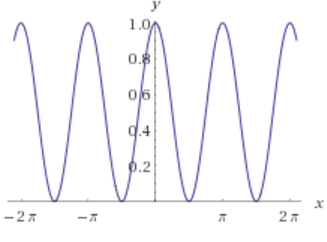
\includegraphics[width=.4\textwidth]{./pictures/15_6_2.png}
  \caption{График функции $ \cos^2 t$}
  \label{fig:1562}
\end{figure}

Теорема Пойа не подходит, но $ \cos t$ является характеристической функцией.
Пусть $ \xi_1, \dotsc, \xi_n$ --- независимые случайные величины.
Тогда
$$ \varphi_{ \xi_1 + \xi_2 + \dotsc + \xi_n} \left( t \right) =
  \varphi_{ \xi_1} \left( t \right) \cdot \varphi_{ \xi_2} \left( t \right) \cdot \dotsc \cdot
  \varphi_{ \xi_n} \left( t \right).$$

Пусть $ \xi_2, \, \xi_2$ --- независимые случайные величины с распределением
$$P \left( \xi_1 = 1 \right) =
  P \left( \xi_2 = - 1 \right) =
  \frac{1}{2}.$$
Тогда характеристическая функция их суммы
$ \varphi_{ \xi_1 + \xi_2} \left( t \right) =
  \varphi_{ \xi_1} \left( t \right) \cdot \varphi_{ \xi_2} \left( t \right) $.
Из задачи 15.3 $ \varphi_{ \xi_1 + \xi_2} \left( t \right) = \cos^2 t$.
Предъявили ту случайную величину, для которой это является характеристической функцией.

\item нарисуем график функции (рис. \ref{fig:1561}).

\begin{figure}[h!]
  \centering
  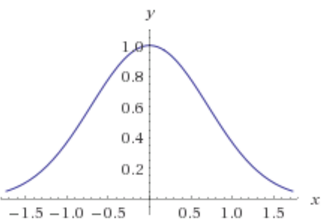
\includegraphics[width=.4\textwidth]{./pictures/15_6_1.png}
  \caption{График функции $e^{- t^2}$}
  \label{fig:1561}
\end{figure}

Это характеристическая функция случайной величины $ \xi \sim N \left( 0, 2 \right) $;

\item используем теорему Пойа.
Нарисуем график (рис. \ref{fig:156}).

\begin{figure}[h!]
  \centering
  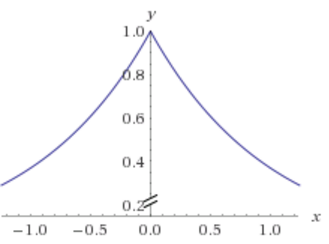
\includegraphics[width=.4\textwidth]{./pictures/15_6.png}
  \caption{График функции $e^{ - \left| t \right| }$}
  \label{fig:156}
\end{figure}

В нуле --- единица, функция чётная, неотрицательная, выпуклая вниз, стремится к нулю.
По теореме Пойа эта функция является характеристической.
\end{enumerate}

\subsubsection*{15.7}

\textit{Задание.} Докажите, что следующие функции не могут быть характеристическими:
\begin{enumerate}[label=\alph*)]
\item $e^{- i \left| t \right| }$;
\item $ \cos t^2$.
\end{enumerate}

\textit{Решение.}
\begin{enumerate}[label=\alph*)]
\item $e^{- i \left| t \right| } = \varphi \left( t \right)$.

Проверим сопряжённость.

$$e^{- i \left| t \right| \neq e^{i \left| - t \right| }}.$$
Отсюда следует, что нарушается условие комплексной сопряжённости;
\item схематически нарисуем график этой функции (рис. \ref{fig:157}).

\begin{figure}[h!]
  \centering
  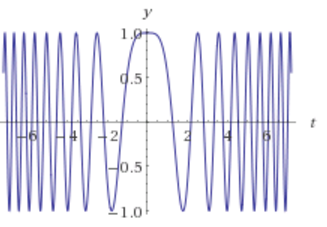
\includegraphics[width=.4\textwidth]{./pictures/15_7.png}
  \caption{График функции $ \cos t^2$}
  \label{fig:157}
\end{figure}

Нарушается равномерная непрерывность.

Покажем это.

Покажем, что размах --- 2.
Берём $t_1 = \sqrt{2k \pi }$, а $t_2 = \sqrt{2k \pi + \pi }$.
Смотрим на их разность
$$ \left| t_2 - t_1 \right| =
\frac{ \pi }{ \sqrt{2k \pi } + \sqrt{2k \pi + \pi }}.$$

Когда $k \rightarrow \infty $, то $ \left| t_2 - t_1 \right| \rightarrow 0$.
Значит можем найти как угодно близкие точки.
Смотрим на разность значений функций в этих точках
$ \left| \varphi \left( t_2 \right) - \varphi \left( t_1 \right) \right| =
  \left| 1 - \left( -1 \right) \right| =
  2$.

Расстояние равно двум, остаётся постоянным, к нулю не стремится.
\end{enumerate}

\subsubsection*{15.8}

\textit{Задание.}
Докажите, что если $ \varphi \left( t \right) $ является характеристической функцией,
то $ \left| \varphi \left( t \right) \right|^2$ тоже есть характеристической функцией.

\textit{Решение.}
$ \left| \varphi \left( t \right) \right|^2 =
  \varphi \left( t \right) \overline{ \varphi \left( t \right) }$.
По одному из свойств это равно $ \varphi \left( t \right) \varphi \left( - t \right) $.

По определению характеристической функции $ \varphi \left( t \right) = Me^{it \xi }$.

Тогда
$ \varphi \left( - t \right) =
  Me^{- it \xi } =
  Me^{it \left( - \xi \right) } =
  \varphi_{- \xi } \left( t \right) $.

Пусть $ \xi_1, \, \xi_2$ ---
независимые случайные величины с характеристической функцией
$ \varphi \left( t \right) =
  \varphi_{ \xi_1} \left( t \right) =
  \varphi_{ \xi_2} \left( t \right) $.

Тогда
$ \varphi_{ \xi_1 - \xi_2} \left( t \right) =
  \varphi_{ \xi_1} \left( t \right) \varphi_{- \xi} \left( t \right) =
  \varphi_{ \xi_1} \left( t \right) \varphi_{ \xi_2} \left( - t \right) $.
Это одна и та же характеристическая функция,
потому это равно $ \varphi \left( t \right) \varphi \left( - t \right) $.

\subsubsection*{15.9}

\textit{Задание.}
Используя характеристические функции, докажите, что если $ \xi_1, \, \xi_2$ ---
независимые случайные величины,
которые имеют нормальные распределения
$N \left( a_1, \sigma_1^2 \right) $ и $N \left( a_2, \sigma_2^2 \right) $ соответственно,
то случайная величина $ \xi_1 + \xi_2$ имеет нормальное распределение
$N \left( a_1 + a_1, \sigma_1^2 + \sigma_2^2 \right) $.

\textit{Решение.}
$ \xi_1 \sim N \left( a_1, \sigma_1^2 \right), \,
  \xi_2 \sim N \left( a_2, \sigma_2^2 \right) $.

Характеристические функции этих случайных величин соответственно равны
$ \varphi_{ \xi_1} \left( t \right) = e^{ita_1 - \frac{t^2 \sigma_1^2}{2}}, \,
\varphi_{ \xi_2} \left( t \right) = e^{ita_2 - \frac{t^2 \sigma_2^2}{2}}$.

Найдём характеристическую функцию суммы.
$ \xi_1, \, \xi_2$ --- независимы.
Поэтому
$ \varphi_{ \xi_1 + \xi_2} \left( t \right) =
\varphi_{ \xi_1} \left( t \right) \varphi_{ \xi_2} \left( t \right) =
e^{it \left( a_1 + a_2 \right) - \frac{t^2}{2} \left( \sigma_1^2 + \sigma_2^2 \right) }$.
Из этого следует, что $ \xi_1 + \xi_2 \sim N \left( a_1 + a_1, \sigma_1^2 + \sigma_2^2 \right) $.

\subsubsection*{15.10}

\textit{Задание.}
Пусть $ \xi_1, \, \xi_2$ --- независимые случайные величины,
каждая из которых имеет стандартное нормальное распределение.
Вычислите характеристическую функцию случайной величины
$$ \eta =
\frac{ \xi_1^2 - \xi_2^2}{2}.$$

\textit{Решение.}
$ \xi_1, \, \xi_2$ ---
независимые случайные величины со стандартным нормальным распределением
$ \xi_1 \sim N \left( 0, 1 \right), \,
  \xi_2 \sim N \left( 0, 1 \right) $.

Их характеристические функции
$ \varphi_{ \xi_1} \left( t \right) =
  \varphi_{ \xi_2} \left( t \right) =
  e^{- \frac{t^2}{2}}$.

Нужно найти характеристическую функцию случайной величины
$$ \eta =
  \frac{ \xi_1^2 - \xi_2^2}{2} =
  \frac{ \xi_1^2}{2} - \frac{ \xi_2^2}{2}.$$

Воспользовавшись свойством
$ \varphi_{a \xi } \left( t \right) =
  Me^{i \left( ta \right) \xi } =
  \varphi_{ \xi } \left( at \right) $
получим
$$ \varphi_{ \eta } \left( t \right) =
  \varphi_{ \xi_1^2 - \xi_2^2} \left( \frac{t}{2} \right).$$
Пользуемся независимостью
$$ \varphi_{ \xi_1^2 - \xi_2^2} \left( \frac{t}{2} \right) =
  \varphi_{ \xi_1^2} \left( \frac{t}{2} \right) \cdot
  \varphi_{- \xi_2^2} \left( \frac{t}{2} \right) -
  \varphi_{ \xi_1^2} \left( \frac{t}{2} \right) \cdot
  \varphi_{ \xi_2^2} \left( - \frac{t}{2} \right).$$

Найдём характеристическую функцию квадрата случайной величины по определению
$$ \varphi_{ \xi_2^2} \left( \frac{t}{2} \right) =
  Me^{i \cdot \frac{t}{2} \cdot \xi_1^2} =
  \int \limits_{- \infty }^{+ \infty } e^{i \cdot \frac{t}{2} \cdot x^2} \cdot
  \frac{1}{ \sqrt{2 \pi }} \cdot e^{- \frac{x^2}{2}}dx =
  \frac{1}{ \sqrt{2 \pi }} \int \limits_{- \infty }^{ \infty }
  e^{- \frac{x^2}{2} \left( 1 - it \right) }dx.$$
Делаем замену $y = x \sqrt{1 - it}, dy = \sqrt{1 - it}dt$.
Получаем
$$ \frac{1}{ \sqrt{2 \pi }}
  \int \limits_{- \infty }^{ \infty } e^{- \frac{x^2}{2} \left( 1 - it \right) }dx =
  \frac{1}{ \sqrt{2 \pi }}
  \int \limits_{- \infty }^{ \infty } e^{- \frac{y^2}{2}} \cdot \frac{1}{ \sqrt{1 - it}} dy.$$
В силу того, что
$$ \int \limits_{- \infty }^{ \infty }p \left( x \right) dx =
  1,$$
получаем, что
$$ \frac{1}{ \sqrt{2 \pi }} \int \limits_{- \infty }^{ \infty } e^{- \frac{y^2}{2}}dy =
  1.$$
Остаётся
$$ \frac{1}{ \sqrt{2 \pi }}
  \int \limits_{- \infty }^{ \infty } e^{- \frac{y^2}{2}} \cdot \frac{1}{ \sqrt{1 - it}} dy =
  \frac{1}{ \sqrt{1 - it}}.$$

В итоге получаем
$$ \varphi_{ \eta } \left( t \right) =
  \varphi_{ \xi_1^2} \left( \frac{t}{2} \right) \cdot
  \varphi_{ \xi_2^2} \left( - \frac{t}{2} \right) =
  \frac{1}{ \sqrt{1 - it}} \cdot \frac{1}{ \sqrt{1 - it}} =
  \frac{1}{ \sqrt{1 + t^2}}.$$

\subsubsection*{15.11}

\textit{Задание.}
Пусть $ \left\{ \xi_n \right\}_{n \geq 1}$ ---
последовательность независимых одинаково распределённых случайных величин с характеристической
функцией $ \varphi $,
и пусть $ \nu $ --- случайная величина, которая не зависит от $ \left\{ \xi_n \right\}_{n \geq 1}$,
и принимает целые неотрицательные значения: $P \left( \nu = k \right) = p_k$.
\begin{enumerate}[label=\alph*)]
\item Найдите характеристическую функцию случайной величины $ \xi_1 + \dotsc + \xi_{ \nu }$;
\item для какой случайной величины функция
$$ \frac{1}{2 - \varphi \left( t \right) }$$
является характеристической?
\end{enumerate}

\textit{Решение.}
\begin{enumerate}[label=\alph*)]
\item
Ищем по определению
$ \varphi_{ \xi_1 + \dotsc + \xi_{ \nu }} \left( t \right) =
  Me^{it \left( \xi_1 + \dotsc + \xi_n \right) }$.
Нужно ввести все возможные значения $ \nu $.
Получим
$$ \varphi_{ \xi_1 + \dotsc + \xi_{ \nu }} \left( t \right) =
  M \left[
    \sum \limits_{n=0}^{ \infty }
      \mathbbm{1} \left( \nu = n \right) e^{it \left( \xi_1 + \dotsc + \xi_n \right) }
  \right].$$
Обозначим
$$ \sum \limits_{n=0}^{ \infty }
    \mathbbm{1} \left( \nu = n \right) e^{it \left( \xi_1 + \dotsc + \xi_n \right) } =
  S.$$
Отличное от нуля в этой сумме одно слагаемое.
Берём частичную сумму
$$S_m =
  \sum \limits_{n=0}^m \mathbbm{1}
    \left( \nu = n \right) e^{it \left( \xi_1 + \dotsc + \xi_n \right) } \rightarrow
  S, \,
  m \rightarrow \infty.$$

Оценим
$$ \left| S_m \right| \leq
  \sum \limits_{n=0}^m
  \left|
    \mathbbm{1} \left( \nu = n \right) e^{it \left( \xi_1 + \dotsc + \xi_n \right) }
  \right| \leq
  \sum \limits_{n=0}^m \mathbbm{1} \left( \nu = n \right).$$

Теперь нужно убедиться, что математическое ожидание этой суммы --- конечное.
Пользуемся линейностью
$$M \sum \limits_{n=0}^m \mathbbm{1} \left( \nu = n \right) =
  \sum \limits_{n=0}^m P \left( \nu = n \right) =
  \sum \limits_{n=0}^m p_n \leq
  1,$$
потому что это распределение случайной величины.
Из этого следует, что
$$MS =
  \lim \limits_{m \to \infty } MS_m.$$

Вернёмся к характеристической функции и пользуемся независимостью
$ \nu $ и $ \left\{ \xi_n \right\}_{n \geq 1}$.
Получаем
\begin{equation*}
\begin{split}
\varphi_{ \xi_1 + \dotsc + \xi_{ \nu }} \left( t \right) =
  MS =
  \sum \limits_{n=0}^{ \infty }
    M \mathbbm{1} \left( \nu = n \right) Me^{it \left( \xi_1 + \dotsc + \xi_n \right) } = \\
  = \sum \limits_{n=0}^{ \infty } p_n \varphi_{ \xi_1 + \dotsc + \xi_n} \left( t \right).
\end{split}
\end{equation*}
Пользуемся независимостью
$$ \varphi_{ \xi_1 + \dotsc + \xi_{ \nu }} \left( t \right) =
  \sum \limits_{n=0}^{ \infty } p_n \varphi_{ \xi_1 + \dotsc + \xi_n} \left( t \right) =
  \sum \limits_{n=0}^{ \infty } p_n \varphi^n \left( t \right).$$
\item есть последовательность $ \left\{ \xi_n \right\}_{n = 1}^{ \infty }$
независимых одинаково распределённых случайных величин с характеристической функцией $ \varphi $.

Случайная величина $ \nu $ не зависит от $ \xi_1, \dotsc, \xi_n, \dotsc $ и имеет распределение
$P \left\{ \nu = k \right\} = p_k, \,
  k \geq 0$.

Тогда характеристическая функция $ \eta = \xi_1 + \dotsc + \xi_{ \nu }$ выглядела так
$$ \varphi_{ \eta } \left( t \right) =
  \sum \limits_{k = 0}^{ \infty } \varphi^k \left( t \right) \cdot p_k.$$

Какая случайная величина может иметь характеристическую функцию
$$ \frac{1}{2 - \varphi \left( t \right) } =
  \frac{1}{2} \cdot \frac{1}{1 - \frac{ \varphi \left( t \right) }{2}}.$$
Применяем формулу для суммы геометрической прогрессии
$$ \frac{1}{2 - \varphi \left( t \right) } =
  \frac{1}{2}
  \sum \limits_{k = 0}^{ \infty } \left( \frac{ \varphi \left( t \right) }{2} \right)^k =
  \sum \limits_{k = 0}^{ \infty } \varphi^k \left( t \right) \cdot \frac{1}{2^{k+1}}.$$

Если положим
$$p_k = \frac{1}{2^{k+1}}, \,
  k \geq 0,$$
то
$$ \frac{1}{2 - \varphi \left( t \right) }$$
будет характеристической функцией $ \eta $.
\end{enumerate}

\subsubsection*{15.12}

\textit{Задание.}
Пусть $ \left\{ \xi_n \right\}_{n \geq 1}$ ---
последовательность независимых одинаково распределённых случайных величин с равномерным
распределением на $ \left[ 0, 1 \right] $, и пусть $ \nu $ --- случайная величина,
которая не зависит от $ \left\{ \xi_n \right\}_{n \geq 1}$,
и имеет распределение Пуассона с параметром $ \lambda $.
Докажите, что случайная величина
$$ \eta \left( t \right) =
  \sum \limits_{k = 1}^{ \nu } \mathbbm{1} \left\{ \xi_k \in \left[ 0, t \right] \right\} $$
имеет распределение Пуассона с параметром $ \lambda t$.

\textit{Решение.}
$ \left\{ \xi_n \right\}_{n \geq 1}$ ---
последовательность независимых одинаково распределённых случайных величин с плотностью распределения
$$p_{ \xi_n} \left( x \right) = \mathbbm{1}_{ \left[ 0, 1 \right] } \left( x \right), \,
  n \geq 1.$$

Случайная величина $ \nu $ ---
независима от $ \left\{ \xi_n \right\}_{n \geq 1}$ и имеет распределение
$$P \left( \nu = k \right) =
  \frac{ \lambda^k}{k!} \cdot e^{- \lambda }.$$

Есть случайная величина
$$ \nu \left( t \right) =
  \sum \limits_{k = 1}^{ \nu } \mathbbm{1} \left\{ \xi_k \in \left[ 0, t \right] \right\}, \,
  t > 0.$$

По определению
$$ \varphi_{ \eta } \left( z \right) =
  Me^{iz \eta } =
  Me^{iz \left( \mathbbm{1} \left\{ \xi_1 \in \left[ 0, t \right] \right\} + \dotsc +
    \mathbbm{1} \left\{ \xi_{ \nu } \in \left[ 0, t \right] \right\} \right) } =
  M \sum \limits_{k = 0}^{ \infty }
    \left[ \mathbbm{1} \left( \nu = k \right) e^{iz \eta } \right].$$
Запишем в явном виде случайную величину $ \eta $.
Получим
$$ \varphi_{ \eta } \left( z \right) =
  M \sum \limits_{k = 0}^{ \infty } \left( \mathbbm{1} \left\{ \nu = k \right\}
  e^{iz \sum \limits_{j = 1}^{ \nu }
    \mathbbm{1} \left\{ \xi_j \in \left[ 0, t \right] \right\} } \right).$$
Поменяем знак суммы и математического ожидания и воспользуемся тем,
что математическое ожидание произведения независимых случайных величин равно произведению их
математических ожиданий
$$ \varphi_{ \eta } \left( z \right) =
  \sum \limits_{k = 0}^{ \infty } M \left[ \mathbbm{1} \left( \nu = k \right) \right]
  Me^{iz \sum \limits_{j = 1}^{ \nu }
    \mathbbm{1} \left\{ \xi_j \in \left[ 0, t \right] \right\} }.$$
Математическое ожидание индикатора события --- это вероятность данного события
$$ \varphi_{ \eta } \left( z \right) =
  \sum \limits_{k = 0}^{ \infty }
    P \left( \nu = k \right)
    Me^{iz \sum \limits_{j = 1}^k \mathbbm{1} \left\{ \xi_j \in \left[ 0, t \right] \right\} } =
  \sum \limits_{k = 0}^{ \infty } \frac{ \lambda^k}{k!} \cdot e^{- \lambda }
  \prod \limits_{j = 1}^k
    Me^{iz \cdot \mathbbm{1} \left\{ \xi_j \in \left[ 0, t \right] \right\} }.$$
Случайные величины независимы и одинаково распределены
$$  \varphi_{ \eta } \left( z \right) =
  \sum \limits_{k = 0}^{ \infty }
    \frac{ \lambda^k}{k!} \cdot e^{- \lambda}
    \left( Me^{iz \cdot \mathbbm{1} \left\{ \xi_1 \in \left[ 0, t \right] \right\} } \right)^k.$$

Найдём математическое ожидание из полученного выражения
$$Me^{iz \cdot \mathbbm{1} \left\{ \xi_1 \in \left[ 0, t \right] \right\} } =
  te^{iz} + \left( 1 - t \right) =
  t \left( e^{iz} - 1 \right) + 1.$$

Тогда характеристическая функция равна
$$ \varphi_{ \eta } \left( z \right) =
  \sum \limits_{k = 0}^{ \infty }
    \frac{ \lambda^k}{k!} \cdot e^{- \lambda } \left[ t \left( e^{iz} - 1 \right) + 1 \right]^k =
  e^{- \lambda }
  \sum \limits_{k = 0}^{ \infty }
    \frac{ \lambda^k}{k!} \left[ t \left( e^{iz} - 1 \right) + 1 \right].$$
Данная сумма --- это ряд для экспоненты, поэтому
$ \varphi_{ \eta } \left( z \right) =
  e^{ \lambda t \left( e^{iz} - 1 \right) }$.

\subsubsection*{15.13}

\textit{Задание.}
С помощью характеристической функции вычислите моменты случайной величины со стандартным нормальным
распределением.

\textit{Решение.} $ \xi \sim N \left( 0, 1 \right) $ имеет плотность распределения
$$p_{ \xi } \left( x \right) =
\frac{1}{ \sqrt{2 \pi }} \cdot e^{- \frac{x^2}{2}}$$
и характеристическую функцию $ \varphi_{ \xi } \left( t \right) = e^{- \frac{t^2}{2}}$.

Моменты случайной величины связаны с характеристической функцией формулой
\begin{equation}\label{eq:connection}
  M \xi^k =
\left( -i \right)^k \varphi^{ \left( k \right) } \left( 0 \right).
\end{equation}

Найдём производную характеристической функции
$ \varphi_{ \xi }' \left( t \right) =
  -te^{- \frac{t^2}{2}}$.

Запишем ряд Тейлора для экспоненты
$$e^x =
  \sum \limits_{k = 0}^{ \infty } \frac{x^k}{k!}.$$

Вместо $x$ подставим $-t^2 / 2$ и получим
$$ \varphi_{ \xi } \left( t \right) =
  e^{- \frac{t^2}{2}} =
  \sum \limits_{k = 0}^{ \infty } \frac{ \left( - \frac{t^2}{2} \right)^k}{k!} =
  \sum \limits_{k = 0}^{ \infty } \frac{ \left( -1 \right)^k t^{2k}}{2^k k!}.$$
Все слагаемые, где $t$ имеют нечётные степени, имеют нулевой коэффициент.

С другой стороны
$$ \varphi \left( t \right) =
  \sum \limits_{k = 0}^{ \infty }
    \frac{ \varphi^{ \left( k \right) \left( 0 \right) }}{k!} \cdot t^k.$$

Приравниваем коэффициенты при соответствующих степенях
$$ \sum \limits_{k = 0}^{ \infty } \frac{ \left( -1 \right)^k t^{2k}}{2^k k!} =
  \sum \limits_{k = 0}^{ \infty }
    \frac{ \varphi^{ \left( 2k \right) } \left( 0 \right) t^{2k}}{ \left( 2k \right)!}.$$

Для нечётных степеней $ \varphi^{ \left( 2k - 1 \right) } \left( 0 \right) = 0$.

Для четных ---
$$ \varphi^{ \left( 2k \right) } \left( 0 \right) =
  \frac{ \left( -1 \right)^k \left( 2k \right)!}{2^k k!}.$$
Представим знаменатель дроби в виде
$$2^k k! =
  \left( 2 \cdot 1 \right) \left( 2 \cdot 2 \right) \cdot \dotsc \cdot \left( k \cdot 2 \right) =
  2 \cdot 4 \cdot \dotsc \cdot \left( 2k \right) =
  \left( 2k \right)!!.$$
Тогда
$$ \varphi^{ \left( 2k \right) } \left( 0 \right) =
  \frac{ \left( -1 \right)^k \left( 2k \right)!}{ \left( 2k \right)!!} =
  \left( -1 \right)^k \left( 2k - 1 \right)!!.$$

Остаётся воспользоваться формулой \eqref{eq:connection}.
$ \left( -i \right)^{2k} =
  \left( -1 \right)^k$.
Отсюда следует,
что
$M \xi^k =
  \left( -1 \right)^k \left( -1 \right)^k \left( 2k - 1 \right)!! =
  \left( 2k - 1 \right)!!$.

\addcontentsline{toc}{section}{Домашнее задание}
\section*{Домашнее задание}

\subsubsection*{15.17}

\textit{Задание.}
Пусть $ \xi_1, \dotsc, \xi_n$ --- независимые случайные величины,
каждая из которых принимает значения $1$ и $- 1$ с вероятностью $1 / 2$.
Найдите характеристическую функцию случайной величины $S_n = \xi_1 + \dotsc + \xi_n$.

\textit{Решение.} Найдём характеристическую функцию каждой из случайных величин
$$ \varphi_{ \xi_1} \left( t \right) =
  \dotsc =
  \varphi_{ \xi_n} \left( t \right) =
  \varphi_{ \xi } \left( t \right) =
  Me^{it \xi } =
  e^{it} \cdot \frac{1}{2} + e^{- it} \cdot \frac{1}{2} =
  \frac{1}{2} \left( e^{it} + e^{- it} \right) =
  \cos t.$$

Так как случайные величины $ \xi_1, \dotsc, \xi_n$ --- независимы,
то
$ \varphi_{S_n} \left( t \right) = \\
  = \varphi_{ \xi_1 + \dotsc + \xi_n} \left( t \right) =
  Me^{it \left( \xi_1 + \dotsc + \xi_n \right) } =
  Me^{it \xi_1} \dotsc e^{it \xi_n} =
  \varphi_{ \xi_1} \left( t \right) \dotsc \varphi_{ \xi_n} \left( t \right) = \\
  = \varphi_{ \xi}^n \left( t \right) =
  \cos^n \left( t \right) $.

\subsubsection*{15.18}

\textit{Задание.} Докажите, что следующие функции являются характеристическими:
\begin{enumerate}[label=\alph*)]
\item $e^{- \left| t \right| } \cos t$;
\item $ \left( 1 + e^{- \left| t \right| }e^{- t^2} \right) / 2$.
\end{enumerate}

\textit{Решение.}
\begin{enumerate}[label=\alph*)]
\item Рассмотрим функцию $e^{- \left| t \right| }$.
Её график изображён на рисунке \ref{fig:156}.
Из рисунка видим, что функция в нуле равна единице, неотрицательная, чётная,
выпуклая вниз на интервале $ \left[ 0, + \infty \right) $, непрерывна,
стремится к нулю на бесконечности.
По теореме Пойа эта функция является характеристической.
Это характеристическая функция случайной величины $ \xi_1$, имеющей распределение Коши.

Из задачи 15.17 функция $ \cos t$ является характеристической функцией для случайной величины,
которая принимает значения 1 и $- 1$ с вероятностью $1 / 2$.

Пусть $ \xi_1, \, \xi_2, \dotsc, \xi_n$ --- независимые случайные величины.
Тогда
$$ \varphi_{ \xi_1 + \xi_2 + \dotsc + \xi_n} \left( t \right) =
  \varphi_{ \xi_1} \left( t \right) \cdot \varphi_{ \xi_2} \left( t \right) \cdot \dotsc \cdot
  \varphi_{ \xi_n} \left( t \right).$$
Пусть $ \xi_1, \, \xi_2$ --- независимые случайные величины,
первая из которых имеет распределение Коши, а вторая ---
$$P \left\{ \xi_2 = 1 \right\} =
  P \left\{ \xi_2 = - 1 \right\} =
  \frac{1}{2}.$$
Тогда характеристическая функция их суммы
$$ \varphi_{ \xi_1 + \xi_2} \left( t \right) =
  \varphi_{ \xi_1} \left( t \right) \cdot \varphi_{ \xi_2} \left( t \right) =
  e^{- \left| t \right| } \cos t.$$
Предъявили ту случайную величину, для которая заданная функция является характеристической;
\item $e^{- \left| t \right| }$ ---
характеристическая функция случайной величины $ \xi_1$ с распределением Коши.
$e^{- t^2}$ --- характеристическая функция случайной величины $ \xi_2 \sim N \left( 0, 2 \right) $,
так как для случайной величины $ \xi \sim N \left( a, \sigma^2 \right) $
характеристическая функция равна
$ \varphi_{ \xi } \left( t \right) =
  e^{ita}e^{- \frac{t^2 \sigma^2}{2}}$.

$ \xi_1$ и $ \xi_2$ --- независимые.
Из этого следует,
что
$ \varphi_{ \xi_1 + \xi_2} \left( t \right) =
  \varphi_{ \xi_1} \left( t \right) \cdot \varphi_{ \xi_2} \left( t \right) =
  e^{- \left| t \right| } e^{- t^2}$,
то есть $e^{- \left| t \right| } e^{- t^2}$ ---
характеристическая функция для случайной величины $ \left( \xi_1 + \xi_2 \right) $.

Пусть случайная величина $ \eta $ имеет распределение
$$ \eta =
  \begin{cases}
    \xi_1 + \xi_2, \qquad \frac{1}{2}, \\
    0, \qquad \frac{1}{2}.
  \end{cases}$$
Тогда её характеристическая функция равна
$$ \varphi_{ \eta } \left( t \right) =
  Me^{it \eta } =
  Me^{it \left( \xi_1 + \xi_2 \right) } \cdot \frac{1}{2} + \frac{1}{2} \cdot Me^{it \cdot 0} =
  \frac{1}{2} \cdot M1 + \frac{1}{2} \cdot Me^{it \xi_1} Me^{it \xi_2}.$$
По определению характеристической функции и свойствам математического ожидания получаем
$$ \varphi_{ \eta } \left( t \right) =
  \frac{1}{2} \cdot 1 +
  \frac{1}{2} \cdot \varphi_{ \xi_1} \left( t \right) \varphi_{ \xi_2} \left( t \right) =
  \frac{1}{2} + \frac{1}{2} \cdot e^{- \left| t \right| }e^{- t^2} =
  \frac{1 + e^{- \left| t \right| }e^{- t^2}}{2}.$$
Предъявили случайную величину, для которой заданная функция является характеристической.
\end{enumerate}

\subsubsection*{15.19}

\textit{Задание.} Докажите, что следующие функции не могут быть характеристическими:
\begin{enumerate}[label=\alph*)]
\item
  $a_1 \cos t + \dotsc + a_n \cos nt + b_1 \sin t + \dotsc + b_n \sin nt; \,
  b_1 \cdot \dotsc \cdot b_n \neq 0, \, a_i, \, b_i \in \mathbb{R}$;
\item $e^t$;
\item $ \cos t^3$.
\end{enumerate}

\textit{Решение.}
\begin{enumerate}[label=\alph*)]
\item Проверим свойство комплексной сопряжённости.
Должно быть
$$ \varphi \left( t \right) =
  \overline{ \varphi \left( - t \right) }.$$
Найдём
$ \varphi \left( - t \right) =
  a_1 \cos \left( - t \right) + \dotsc + a_n \cos \left( - nt \right) +
  b_1 \sin \left( - t \right) + \dotsc + \\
  + b_n \sin \left( - nt \right) =
  a_1 \cos t + \dotsc + a_n \cos \left( nt \right) - b_1 \sin t - \dotsc -
  b_n \sin \left( nt \right) = \\
  = \overline{ \varphi \left( - t \right) }$,
так как функция действительная.
Получили, что
$$ \varphi \left( t \right) \neq
  \overline{ \varphi \left( - t \right) },$$
то есть нарушается условие комплексной сопряжённости;
\item проверим свойство комплексной сопряжённости.
Должно быть
$$ \varphi \left( t \right) =
  \overline{ \varphi \left( - t \right) }.$$
Найдём $ \varphi \left( - t \right) = e^{-t} = \overline{ \varphi \left( - t \right) }$,
так как функция действительная.
Получили, что $ \varphi \left( t \right) \neq \overline{ \varphi \left( - t \right) }$,
то есть нарушается условие комплексной сопряжённости;
\item схематически нарисуем график этой функции (рис. \ref{fig:1519}).

\begin{figure}[h!]
  \centering
  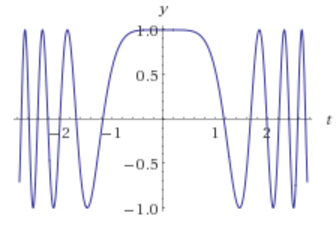
\includegraphics[width=.4\textwidth]{./pictures/15_19.png}
  \caption{График функции $ \cos t^3$}
  \label{fig:1519}
\end{figure}

Покажем, что нарушается равномерная непрерывность.
Берём
$$t_1 = \sqrt[3]{2k \pi }, \,
  t_2 = \sqrt[3]{2k \pi + \pi }.$$
Смотрим на их разность
$$ \left| t_2 - t_1 \right| =
  \left| \sqrt[3]{2k \pi + \pi } - \sqrt[3]{2k \pi } \right|.$$
Умножим и поделим на их неполный квадрат
$$ \left| t_2 - t_1 \right| =
  \frac{2k \pi + \pi - 2k \pi}{ \left( 2k \pi + \pi \right)^{ \frac{2}{3}} + \sqrt[3]{2k \pi + \pi }
  \sqrt[3]{2k \pi } + \left( 2k \pi \right)^{ \frac{2}{3}}}.$$
Первое и последнее слагаемые в числителе уничтожаются
$$ \left| t_2 - t_1 \right| =
  \frac{ \pi }{ \left( 2k \pi + \pi \right)^{ \frac{2}{3}} +
  \sqrt[3]{ \left( 2k \pi + \pi \right) \left( 2k \pi \right) } + \left( 2k \pi \right)^{ \frac{2}{3}}}.$$

Когда $t \rightarrow \infty $, то $ \left| t_2 - t_1 \right| \rightarrow 0$.
Значит можем найти как угодно близкие точки.
Смотрим на разность функций в этих точках
$$ \left| \varphi \left( t_2 \right) - \varphi \left( t_1 \right) \right| =
  \left| \cos \left( 2k \pi + \pi \right) - \cos \left( 2k \pi \right) \right| =
  \left| - 1 - 1 \right| =
  \left| - 2 \right| =
  2.$$

Размах равен двум, остаётся постоянным, к нулю не стремится.
Поэтому функция не является характеристической.
\end{enumerate}

\subsubsection*{15.20}

\textit{Задание.}
Пусть $ \xi $ --- сумма очков, которые выпали при подбрасывании трёх игральных кубиков.
Найдите характеристическую функцию случайной величины $ \xi $.

\textit{Решение.}
Пусть $ \xi_i$ --- случайная величина, которая равна количеству очков, выпавших на $i$-м кубике.
Тогда $ \xi = \xi_1 + \xi_2 + \xi_3$.
На одном кубике может выпасть одно из шести значений с одинаковой вероятностью,
то есть $ \xi_i$ имеет распределение
$$P \left\{ \xi_i = 1 \right\} =
  P \left\{ \xi_i = 2 \right\} =
  \dotsc =
  P \left\{ \xi_i = 6 \right\} =
  \frac{1}{6}, \,
  1 \leq i \leq 3.$$

По определению характеристической функции
$$ \varphi_{ \xi } \left( t \right) =
  Me^{it \xi} =
  Me^{it \left( \xi_1 + \xi_2 + \xi_3 \right) }.$$
Случайные величины $ \xi_1, \, \xi_2$ и $ \xi_3$ --- независимы,
потому характеристическая функция их суммы равна произведению характеристических функций, то есть
$$ \varphi_{ \xi } \left( t \right) =
  \prod \limits_{j = 1}^3 Me^{it \xi_j} =
  \prod \limits_{j = 1}^3 \left( \frac{1}{6} \sum \limits_{k = 1}^6 e^{itk} \right) =
  \frac{1}{216} \left( \sum \limits_{k=1}^6 e^{itk} \right)^3.$$

\subsubsection*{15.21}

\textit{Задание.}
Случайная величина $ \xi $
имеет двухстороннее показательное распределение с плотностью распределения
$$p_{ \xi } \left( x \right) =
  \frac{e^{- \left| x \right| }}{2}, \,
  x \in \mathbb{R}.$$
Докажите, что характеристическая функция $ \xi $ равна
$$ \varphi \left( t \right) =
  \frac{1}{1 + t^2}.$$

\textit{Решение.} Характеристическая функция случайной величины --- это преобразование Фурье плотности:
$$ \varphi \left( t \right) =
  \int \limits_{- \infty }^{+ \infty } e^{itx} \cdot \frac{e^{- \left| x \right| }}{2} dx =
  \int \limits_{- \infty }^0 e^{itx} \cdot \frac{e^x}{2} dx +
  \int \limits_0^{+ \infty } e^{itx} \cdot \frac{e^{- x}}{2} dx.$$
Запишем экспоненты как одну
$$ \varphi \left( t \right) =
  \frac{1}{2} \int \limits_{- \infty }^0 e^{itx + x} dx +
  \frac{1}{2} \int \limits_0^{+ \infty } e^{itx - x} dx =
  \frac{1}{2} \int \limits_{- \infty }^0 e^{x \left( it + 1 \right) } dx +
  \frac{1}{2} \int \limits_0^{+ \infty } e^{x \left( it - 1 \right) }dx.$$
Возьмём интегралы
$$ \varphi \left( t \right) =
  \frac{1}{2} \cdot \left. \frac{1}{it + 1} \cdot
  e^{x \left( it + 1 \right) } \right|_{- \infty }^0 +
  \frac{1}{2} \cdot \left. \frac{1}{it - 1} \cdot
  e^{x \left( it - 1 \right) } \right|_0^{+ \infty }.$$
Подставим пределы интегрирования и приведём к общему знаменателю
$$ \varphi \left( t \right) =
  \frac{1}{2} \cdot \frac{1}{it + 1} - \frac{1}{2} \cdot \frac{1}{it - 1} =
  \frac{1}{2} \cdot \frac{it - 1 - it - 1}{ \left( it + 1 \right) \left( it - 1 \right) } =
  \frac{- 2}{2 \left( - t^2 - 1 \right) } =
  \frac{1}{1 + t^2}.$$

\subsubsection*{15.22}

\textit{Задание.}
Пусть $ \xi_1, \, \xi_2, \dotsc, \xi_n$ --- независимые одинаково распределённые случайные величины,
которые распределены по закону Коши с плотностью
$$p_{ \xi } \left( t \right) =
  \frac{1}{ \pi \left( 1 + x^2 \right) }.$$
Найдите характеристическую функцию случайной величины
$$ \eta =
  \sum \limits_{k=1}^n a_k \xi_k,$$
где $a_1, \dotsc, a_n$ --- неслучайные константы.
Что можно сказать про распределение случайной величины $ \eta $?

\textit{Решение.}
$ \xi_1, \, \xi_2, \dotsc, \xi_n$ --- независимые случайные величины с распределением Коши
$$p \left( x \right) =
  \frac{1}{ \pi \left( 1 + x^2 \right) }.$$

Характеристическая функция --- это преобразование Фурье от функции $p \left( x \right) $.
Найдём её
$$ \varphi \left( t \right) =
  \int \limits_{- \infty }^{+ \infty } \frac{1}{ \pi \left( 1 + x^2 \right) } \cdot e^{itx} dx.$$

Рассмотрим новую функцию
$$f \left( z \right) =
  \frac{e^{itz}}{ \pi \left( 1 + z^2 \right) } =
  \frac{e^{itz}}{ \pi \left( z - i \right) \left( z + i \right) }.$$

Будем считать, что $t > 0$,
в силу свойства комплексной сопряжённости характеристической функции этого достаточно.

Функция $f$ имеет 2 полюса в нулях знаменателя --- точки $ \pm i$ (рис. \ref{fig:1522}).

\begin{figure}[h!]
  \centering
  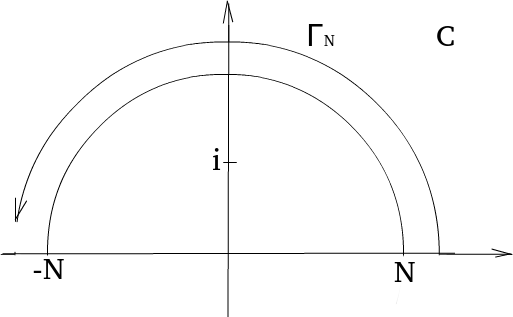
\includegraphics[width=.4\textwidth]{./pictures/15_22.png}
  \caption{Вспомогательный рисунок для нахождения интеграла от функции $f$}
  \label{fig:1522}
\end{figure}

Для больших $N$ есть замкнутый контур с полюсом первого порядка
$$ \int \limits_{ \Gamma_N} f \left( z \right) dz +
\int \limits_{- N}^N \left( rez \, f \right) \left( i \right) =
  2 \pi ie^{- t} \cdot \frac{1}{2i \pi } =
  e^{- t}.$$

В общем случае $ \varphi \left( t \right) = e^{- \left| t \right| }$.

Нужно найти характеристическую функцию случайной величины
$$ \eta =
  \sum \limits_{k = 1}^n a_k \xi_k =
  a_1 \xi_1 + a_2 \xi_2 + \dotsc + a_n \xi_n.$$

Заметим, что
$ \varphi_{a \xi } \left( t \right) =
  Me^{i \left( at \right) \xi } \left( t \right) =
  \varphi_{ \xi } \left( at \right) $.

Из независимости случайных величин следует, что
$$ \varphi_{ \eta } \left( t \right) =
  \varphi_{a_1 \xi_1 + a_2 \xi_2 + \dotsc + a_n \xi_n} \left( t \right) =
  \varphi_{ \xi_1} \left( a_1 t \right) \cdot \varphi_{ \xi_2} \left( a_2 t \right) \cdot
  \dotsc \cdot \varphi_{ \xi_n} \left( a_n t \right) =
  \prod \limits_{k = 1}^n \varphi_{ \xi } \left( a_k t \right).$$
Подставим характеристическую функцию
$$ \varphi_{ \eta } \left( t \right) =
  \prod \limits_{k = 1}^n e^{- \left| a_k t \right| } =
  e^{- \sum \limits_{k = 1}^n \left| a_k t \right| } =
  e^{- \sum \limits_{k = 1}^n \left| a_k \right| \cdot \left| t \right| }.$$

Проверим условие абсолютной интегрируемости характеристической функции
$$ \int \limits_{- \infty }^{+ \infty } \left| \varphi_{ \eta } \left( t \right) \right| dt =
  \int \limits_{- \infty }^{+ \infty }
    \left| e^{- \sum \limits_{k = 1}^n \left| a_k \right| \cdot \left| t \right| } \right| dt.$$
При изменении $t$ на $ \left( - t \right) $ ничего не меняется, значит,
подынтегральная функция чётная
$$ \int \limits_{- \infty }^{+ \infty } \left| \varphi_{ \eta } \left( t \right) \right| dt =
  2 \int \limits_0^{+ \infty } e^{- \sum \limits_{k = 1}^n \left| a_k \right| \cdot t} dt =
  \left. - 2 \cdot \frac{1}{ \sum \limits_{k = 1}^n \left| a_k \right| }
  \cdot e^{- \sum \limits_{k = 1}^n \left| a_k \right| \cdot t} \right|_0^{+ \infty } =
  \frac{2}{ \sum \limits_{k = 1}^n \left| a_k \right| }.$$
При
$$\sum \limits_{k = 1}^n \left| a_k \right| \neq
  0$$
получаем, что
$$ \int \limits_{- \infty }^{+ \infty } \left| \varphi_{ \eta } \left( t \right) \right| dt <
  + \infty.$$
Отсюда следует,
что функция абсолютно интегрируема и можем найти плотность распределения как обратное преобразование
Фурье
$$p_{ \eta } \left( t \right) =
  \frac{1}{2 \pi }
  \int \limits_{- \infty }^{+ \infty }
    e^{- itx} e^{- \sum \limits_{k = 1}^n \left| a_k \right| \cdot \left| t \right| } dt.$$
Раскроем модуль, разбив интеграл на 2
$$p_{ \eta } \left( t \right) =
  \frac{1}{2 \pi }
  \int \limits_{- \infty }^0 e^{- itx} e^{ \sum \limits_{k = 1}^n \left| a_k \right| t} dt +
  \frac{1}{2 \pi }
  \int \limits_0^{+ \infty } e^{- itx} e^{- \sum \limits_{k = 1}^n \left| a_k \right| t} dt.$$
Объединим экспоненты и вынесем $t$ в показателе степени
$$p_{ \eta } \left( t \right) =
  \frac{1}{2 \pi }
  \int \limits_{- \infty }^0
    e^{t \left( \sum \limits_{k = 1}^n \left| a_k \right| - ix \right) } dt +
  \frac{1}{2 \pi }
  \int \limits_0^{+ \infty }
    e^{t \left( - \sum \limits_{k = 1}^n \left| a_k \right| - ix \right) } dt.$$
Возьмём интегралы от экспонент
\begin{equation*}
\begin{split}
  p_{ \eta } \left( t \right) =
  \frac{1}{2 \pi } \cdot \left. \frac{1}{ \sum \limits_{k = 1}^n \left| a_k \right| - ix} \cdot
  e^{t \left( \sum \limits_{k = 1}^n \left| a_k \right| - ix \right) } \right|_{- \infty }^0 - \\
  - \frac{1}{2 \pi } \cdot \left. \frac{1}{ \sum \limits_{k = 1}^n \left| a_k \right| + ix} \cdot
  e^{t \left( - \sum \limits_{k = 1}^n \left| a_k \right| - ix \right) } \right|_0^{+ \infty }.
\end{split}
\end{equation*}
Подставим пределы интегрирования
$$p_{ \eta } \left( t \right) =
  \frac{1}{2 \pi } \cdot
  \frac{1}{ \sum \limits_{k = 1}^n \left| a_k \right| - ix} +
  \frac{1}{2 \pi } \cdot \frac{1}{ \sum \limits_{k = 1}^n \left| a_k \right| + ix} =
  \frac{1}{2 \pi } \cdot
  \frac{ \sum \limits_{k = 1}^n \left| a_k \right| + ix +
  \sum \limits_{k = 1}^n \left| a_k \right| - ix}{ \left( \sum \limits_{k = 1}^n
  \left| a_k \right| \right)^2 + x^2}.$$
Приведём подобные в числителе
$$p_{ \eta } \left( t \right) =
  \frac{1}{2 \pi } \cdot
  \frac{2 \sum \limits_{k = 1}^n
    \left| a_k \right| }{\left( \sum \limits_{k = 1}^n \left| a_k \right| \right)^2 + x^2} =
  \frac{ \sum \limits_{k = 1}^n
    \left| a_k \right| }{ \pi \left[ \left( \sum \limits_{k = 1}^n \left| a_k \right| \right)^2 +
  x^2 \right] }.$$
Отсюда следует, что случайная величина $ \eta $ имеет распределение Коши с параметром
$$ \theta =
  \sum \limits_{k = 1}^n \left| a_k \right|.$$

\subsubsection*{15.23}

\textit{Задание.} Найдите закон распределения, которому соответствует характеристическая функция:
\begin{enumerate}[label=\alph*)]
\item $e^{- \left| t \right| }$;
\item $e^{- t^2}$.
\end{enumerate}

\textit{Решение.}
\begin{enumerate}[label=\alph*)]
\item Проверим абсолютную интегрируемость характеристической функции
$$ \int \limits_{- \infty }^{+ \infty } \left| \varphi \left( t \right) \right| dt =
  \int \limits_{- \infty }^{+ \infty } \left| e^{- \left| t \right| } \right| dt.$$
При замене $t$ на $ \left( - t \right) $ ничего не изменится, значит, подынтегральная функция чётная
$$ \int \limits_{- \infty }^{+ \infty } \left| \varphi \left( t \right) \right| dt =
  2 \int \limits_0^{+ \infty } e^{- t} dt =
  \left. -2e^{- t} \right|_0^{+ \infty } =
  2 <
  + \infty.$$
Из этого следует, что характеристическая функция абсолютно интегрируема,
и можем найти плотность распределения как обратное преобразование Фурье
$$p \left( t \right) =
  \frac{1}{2 \pi } \int \limits_{- \infty }^{+ \infty } e^{- itx} e^{- \left| t \right| } dt =
  \frac{1}{2 \pi }
  \int \limits_{- \infty }^0
    e^{- itx} e^t dt + \frac{1}{2 \pi } \int \limits_0^{+ \infty } e^{- itx} e^{- t} dt.$$
Вынесем $t$ в показателях экспонент
$$p \left( t \right) =
  \frac{1}{2 \pi }
  \int \limits_{- \infty }^0
    e^{t \left( 1 - it \right) } dt + \frac{1}{2 \pi }
  \int \limits_0^{+ \infty } e^{t \left( - 1 - it \right) } dt.$$
Возьмём интегралы
$$p \left( t \right) =
  \frac{1}{2 \pi } \cdot
  \left. \frac{1}{1 - it} \cdot e^{t \left( 1 - it \right) } \right|_{- \infty }^0 +
  \frac{1}{2 \pi } \cdot
  \left. \frac{- 1}{1 + it} \cdot e^{t \left( - 1 - it \right) } \right|_0^{+ \infty }.$$
Подставим пределы интегрирования
$$p \left( t \right) =
  \frac{1}{2 \pi } \cdot \frac{1}{1 - it} + \frac{1}{2 \pi } \cdot \frac{1}{1 + it} =
  \frac{1}{2 \pi } \left( \frac{1}{1 - it} + \frac{1}{1 + it} \right).$$
Приведём к общему знаменателю
$$p \left( t \right) =
  \frac{1}{2 \pi } \cdot \frac{1 + it + 1 - it}{1 + x^2} =
  \frac{2}{2 \pi \left( 1 + x^2 \right) } =
  \frac{1}{ \pi \left( 1 + x^2 \right) };$$
\item проверим абсолютную интегрируемость характеристической функции
$$ \int \limits_{- \infty }^{+ \infty } \left| \varphi \left( t \right) \right| dt =
  \int \limits_{- \infty }^{+ \infty } \left| e^{- t^2} \right| dt =
  \int \limits_{- \infty }^{+ \infty } e^{- t^2} dt.$$

Нужно взять гауссов интеграл, который может быть представлен как
$$I =
  \int \limits_{- \infty }^{+ \infty } e^{- x^2} dx =
  \int \limits_{- \infty }^{+ \infty } e^{- y^2} dy.$$

Рассмотрим квадрат этого интеграла $I^2$.
Вводя двумерные координаты,
переходя от них к полярным координатам
$$ \left( x = r \cos \varphi, \,
  y = r \sin \varphi, \,
  r^2 = x^2 + y^2 \right) $$
и интегрируя по $ \varphi $ (от нуля до $2 \pi $),
получаем
$$I^2 =
  \int \limits_{- \infty }^{+ \infty } \int \limits_{- \infty }^{+ \infty }
    e^{- \left( x^2 + y^2 \right) } dxdy =
  \int \limits_0^{2 \pi } d \varphi \int \limits_0^{+ \infty } e^{- r^2} rdr =
  2 \pi \int \limits_0^{+ \infty } e^{- r^2} dr^2 \cdot \frac{1}{2}.$$
Сократим константы и возьмём интеграл
$$I^2 =
  \pi \left. \cdot e^{- r^2} \right|_0^{+ \infty } =
  \pi.$$

Следовательно,
$$I =
  \int \limits_{- \infty }^{+ \infty } e^{- t^2} dt =
  \sqrt{ \pi } <
  + \infty.$$
Отсюда следует, что характеристическая функция абсолютно интегрируема,
и можем найти плотность распределения как обратное преобразование Фурье
$$p \left( t \right) =
  \frac{1}{2 \pi } \int \limits_{- \infty }^{+ \infty } e^{- itx} e^{- t^2} dt.$$
Выделим полный квадрат в степени экспоненты
\begin{equation*}
\begin{split}
  p \left( t \right) =
  \frac{1}{2 \pi }
  \int \limits_{- \infty }^{+ \infty }
    e^{- \left[ t^2 + itx \cdot 2 \cdot \frac{1}{2} + \frac{1}{4} \left( ix \right)^2 \right] +
    \frac{1}{4} \left( ix \right)^2} dt = \\
  = \frac{1}{2 \pi }
  \int \limits_{- \infty }^{+ \infty }
    e^{- \left( t + \frac{1}{2} \cdot ix \right)^2 - \frac{x^2}{4}} dt.
\end{split}
\end{equation*}
Сделаем замену
$$t + \frac{1}{2} \cdot ix = u, \,
  du = dt.$$
Получим
$$p \left( t \right) =
  \frac{1}{2 \pi } \cdot e^{- \frac{x^2}{4}} \int \limits_{- \infty }^{+ \infty } e^{- u^2} du =
  \frac{1}{2 \pi } \cdot e^{- \frac{x^2}{4}} \cdot \sqrt{ \pi } =
  \frac{e^{- \frac{x^2}{4}}}{2 \sqrt{ \pi }}.$$
\end{enumerate}

\subsubsection*{15.24}

\textit{Задание.}
Пусть $ \xi $ и $ \eta $ --- независимые случайные величины,
причём $ \xi $ имеет равномерное на отрезке $ \left[ 0, 1 \right] $ распределение,
а $ \eta $ распределена по закону Пуассона с параметром $ \lambda $.
Найдите характеристическую функцию случайной величины $ \xi + \eta $.

\textit{Решение.}
$ \xi $ имеет плотность распределения
$p_{ \xi } \left( t \right) =
  \mathbbm{1}_{ \left[ 0, 1 \right] } \left( x \right) $.
Тогда
$$ \varphi_{ \xi } \left( t \right) =
  \int \limits_0^1 e^{itx} dx =
  \left. \frac{1}{it} \cdot e^{itx} \right|_0^1 =
  \frac{1}{it} \left( e^{it} - 1 \right).$$

Случайная величина $ \eta $ имеет пуассоновское распределение с параметром $ \lambda > 0$,
которое выглядит следующим образом
$$P \left\{ \eta = k \right\} =
  e^{- \lambda } \cdot \frac{ \lambda^k}{k!}.$$

Так что
$$ \varphi_{ \eta } \left( t \right) =
  \sum \limits_{k = 0}^{ \infty }
    e^{- \lambda } \cdot \frac{ \lambda^k \left( e^{it} \right)^k}{k!} =
  e^{- \lambda } \sum \limits_{k = 0}^{ \infty } \frac{ \left( \lambda e^{it} \right)^k}{k!} =
  e^{- \lambda } e^{ \lambda e^{it}} =
  e^{ \lambda e^{it} - \lambda } =
  e^{ \lambda \left( e^{it} - 1 \right) }.$$

Так как случайные величины $ \xi $ и $ \eta $ --- независимы, то
$$ \varphi_{ \xi + \eta } \left( t \right) =
  \varphi_{ \xi } \left( t \right) \varphi_{ \eta } \left( t \right) =
  \frac{1}{it} \left( e^{it} - 1 \right) e^{ \lambda \left( e^{it} - 1 \right) }.$$

\subsubsection*{15.25}

\textit{Задание.}
Используя характеристические функции, докажите, что если $ \xi_1, \, \xi_2$ ---
независимые случайные величины,
которые имеют распределение Пуассона с параметрами $ \lambda_1$ и $ \lambda_2$ соответственно,
то случайная величина $ \xi_1 + \xi_2$ имеет распределение Пуассона с параметром
$ \lambda_1 + \lambda_2$.

\textit{Решение.}
$ \xi_1, \, \xi_2$ ---
случайные величины с пуассоновским распределением
$ \xi_1 \sim Pois \left( \lambda_1 \right), \,
  \xi_2 \sim Pois \left( \lambda_2 \right) $.

Их характеристические функции
$ \varphi_{ \xi_1} \left( t \right) = e^{ \lambda_1 \left( e^{it} - 1 \right) }, \,
  \varphi_{ \xi_2} \left( t \right) = e^{- \lambda_2 \left( e^{it} - 1 \right) }$.

Найдём характеристическую функцию суммы случайных величин.

$ \xi_1, \, \xi_2$ --- независимы.
Поэтому
$$ \varphi_{ \xi_1 + \xi_2} \left( t \right) =
  \varphi_{ \xi_1} \left( t \right) \varphi_{ \xi_2} \left( t \right) =
  e^{ \lambda_1 \left( e^{it} - 1 \right) } e^{ \lambda_2 \left( e^{it} - 1 \right) } =
  e^{ \lambda_1 \left( e^{it} - 1 \right) + \lambda_2 \left( e^{it} - 1 \right) }.$$
Вынесем общий множитель в показателе экспоненты за скобки
$$ \varphi_{ \xi_1 + \xi_2} \left( t \right) =
  e^{ \left( e^{it} - 1 \right) \left( \lambda_1 + \lambda_2 \right) }.$$
Из этого следует,
что $ \left( \xi_1 + \xi_2 \right) \sim Pois \left( \lambda_1 + \lambda_2 \right) $.

\subsubsection*{15.26}

\textit{Задание.}
Используя характеристические функции, докажите, что если $ \xi_1, \, \xi_2$ ---
независимые случайные величины,
которые имеют биномиальное распределение с параметрами $ \left( n_1, p \right) $ и
$ \left( n_2, p \right) $ соответственно,
то случайная величина $ \xi_1 + \xi_2$ имеет биномиальное распределение с параметром
$ \left( n_1 + n_2, p \right) $.

\textit{Решение.}
$ \xi_1, \, \xi_2$ ---
случайные величины с биномиальным распределением
$ \xi_1 \sim Binom \left( n_1, p \right), \,
  \xi_2 \sim Binom \left( n_2, p \right) $.

Для биномиального распределения есть вероятность
$$P \left\{ \xi = k \right\} =
  C_n^k p^k \left( 1 - p \right)^{n - k},$$
где $p \in \left( 0, 1 \right), \, k = \overline{0, n}$.

Тогда
$$ \varphi_{ \xi } \left( t \right) =
  Me^{it \xi } =
  \sum \limits_{k = 0}^{n} C_n^k \left( e^{it} \right)^k p^k \left( 1 - p \right)^{n - k} =
  \sum \limits_{k = 0}^{n} C_n^k \left( e^{it} p \right)^k \left( 1 - p \right)^{n - k}.$$
Применяем формулу для бинома Ньютона
$$ \varphi_{ \xi } \left( t \right) =
  \left[ e^{it} p + \left( 1 - p \right) \right]^n =
  \left( e^{it} p + 1 - p \right)^n =
  \left[ p \left( e^{it} - 1 \right) + 1 \right]^n.$$

Случайные величины $ \xi_1, \, \xi_2$ имеют характеристические функции
$$ \varphi_{ \xi_1 } \left( t \right) = \left[ p \left( e^{it} - 1 \right) + 1 \right]^{n_1}, \,
  \varphi_{ \xi_2 } \left( t \right) = \left[ p \left( e^{it} - 1 \right) + 1 \right]^{n_2}.$$

Найдём характеристическую функцию суммы случайных величин.

$ \xi_1, \, \xi_2$ --- независимы,
поэтому
$$ \varphi_{ \xi_1 + \xi_2} \left( t \right) =
  \varphi_{ \xi_1} \left( t \right) \varphi_{ \xi_2} \left( t \right) =
  \left[ p \left( e^{it} - 1 \right) + 1 \right]^{n_1}
  \left[ p \left( e^{it} - 1 \right) + 1 \right]^{n_2}.$$
При перемножении одинаковых выражений их степени складываются, потому
$$ \varphi_{ \xi_1 + \xi_2} \left( t \right) =
  \left[ p \left( e^{it} - 1 \right) + 1 \right]^{n_1 + n_2}.$$

Из этого следует, что $ \left( \xi_1 + \xi_2 \right) \sim Binom \left( n_1 + n_2, p \right) $.

\subsubsection*{15.27}

\textit{Задание.}
Пусть $ \xi $ --- равномерно распределённая на отрезке $ \left[ 0, 1 \right] $ случайная величина,
а $ \nu $ --- случайная величина,
которая не зависит от $ \xi $ и принимает целые положительные значения:
$P \left( \nu = k \right) =
  p_k$.
Найдите характеристическую функцию случайной величины $ \xi \cdot \nu $.

\textit{Решение.}
Случайная величина $ \xi $ равномерно распределена на отрезке $ \left[ 0, 1 \right] $
и имеет характеристическую функцию
$$ \varphi_{ \xi } \left( t \right) =
  \left( e^{it} - 1 \right) \cdot \frac{1}{it}.$$

По определению
$ \varphi_{ \xi \cdot \nu } \left( t \right) =
  Me^{it \xi \cdot \nu } \left( t \right) =
  M \left( e^{it \xi} \right)^{ \nu }.$
Нужно учесть все возможные значения $ \nu $.
Получаем
$$ \varphi_{ \xi \cdot \nu } \left( t \right) =
  M \sum \limits_{n = 1}^{+ \infty } \mathbbm{1} \left( \nu = n \right) e^{it \xi n}.$$
Обозначим
$$ \sum \limits_{n = 1}^{+ \infty } \mathbbm{1} \left( \nu = n \right) e^{it \xi n} =
  S.$$

Отличное от нуля в этой сумме одно слагаемое.
Берём частичную сумму
$$S_m =
  \sum \limits_{n = 1}^{m} \mathbbm{1} \left( \nu = n \right) e^{it \xi n} \rightarrow S, \,
  m \rightarrow \infty.$$

Оценим
$$ \left| S_m \right| \leq
  \sum \limits_{n = 1}^{+ \infty }
    \left| \mathbbm{1} \left( \nu = n \right) e^{it \xi n} \right| \leq
  \sum \limits_{n = 1}^{+ \infty } \mathbbm{1} \left( \nu = n \right).$$

Теперь нужно убедиться, что эта сумма имеет конечное математическое ожидание.
Пользуемся линейностью
$$M \sum \limits_{n = 1}^{+ \infty } \mathbbm{1} \left( \nu = n \right) =
  \sum \limits_{n = 1}^{+ \infty } P \left( \nu = n \right) =
  \sum \limits_{n = 1}^{+ \infty } p_n \leq
  1,$$
потому что это распределение случайной величины.
Из этого следует, что
$$MS =
  \lim \limits_{m \to \infty } MS_m.$$

Теперь сумму математических ожиданий можно записать как математическое ожидание суммы
$$ \varphi_{ \xi \cdot \nu } \left( t \right) =
  \sum \limits_{n = 1}^{+ \infty } M \mathbbm{1} \left( \nu = n \right) \cdot Me^{it \xi n} =
  \sum \limits_{n = 1}^{+ \infty } p_n \varphi_{ \xi } \left( tn \right) =
  \sum \limits_{n = 1}^{+ \infty } p_n \left( e^{itn} - 1 \right) \cdot \frac{1}{itn}.$$

\subsubsection*{15.28}

\textit{Задание.}
С помощью характеристической функции вычислите моменты случайной величины с распределением$N \left( 0, \sigma^2 \right) $.

\textit{Решение.} $ \xi \sim N \left( 0, \sigma^2 \right) $ имеет характеристическую функцию
$$ \varphi \left( t \right) =
  e^{- \frac{t^2 \sigma^2}{2}}.$$

Моменты случайной величины связаны с характеристической функцией формулой \eqref{eq:connection}.

Запишем ряд Тейлора для экспоненты
$$e^x =
  \sum \limits_{k = 0}^{ \infty } \frac{x^k}{k!}.$$

Вместо $x$ подставим
$$- \frac{t^2 \sigma^2}{2}$$
и получим
$$ \varphi \left( t \right) =
  e^{- \frac{t^2 \sigma^2}{2}} =
  \sum \limits_{k = 0}^{ \infty } \frac{ \left( - \frac{t^2 \sigma^2}{2} \right)^2}{k!} =
  \sum \limits_{k = 0}^{ \infty } \frac{ \left( -1 \right)^k t^{2k} \sigma^{2k}}{2^k k!}.$$

С другой стороны
$$ \varphi \left( t \right) =
  \sum \limits_{k = 0}^{ \infty }
    \frac{ \varphi^{ \left( k \right) } \left( 0 \right) }{k!} \cdot t^k.$$

Приравниваем коэффициенты при соответствующих степенях
$$ \sum \limits_{k = 0}^{ \infty } \frac{ \left( -1 \right)^k t^{2k} \sigma^{2k}}{2^k k!} =
  \sum \limits_{k = 0}^{ \infty }
    \frac{ \varphi^{ \left( 2k \right) } \left( 0 \right) t^{2k}}{ \left( 2k \right)!}.$$

Для нечётных степеней $ \varphi^{ \left( 2k - 1 \right) } \left( 0 \right) = 0$.

Для чётных степеней
$$ \varphi^{ \left( 2k \right) } \left( 0 \right) =
  \frac{ \left( -1 \right)^k \left( 2k \right)! \sigma^{2k}}{2^k k!}.$$

Представим знаменатель дроби в виде
$$2^k k! =
  \left( 2 \cdot 1 \right) \cdot \left( 2 \cdot 2 \right) \cdot \dotsc \cdot
  \left( 2 \cdot k \right) =
  \left( 2k \right)!!.$$

Тогда
$$ \varphi^{ \left( 2k \right) } \left( 0 \right) =
  \frac{ \left( -1 \right)^k \left( 2k \right)! \sigma^{2k}}{ \left( 2k \right)!!} =
  \left( -1 \right)^k \left( 2k - 1 \right)!! \sigma^{2k}.$$

Остаётся воспользоваться формулой \eqref{eq:connection}.

$ \left( -i \right)^{2k} = \left( -1 \right)^k$.
Отсюда следует, что
$$M \xi^k =
  \left( -1 \right)^k \left( -1 \right)^k \left( 2k - 1 \right)!! \sigma^{2k} =
  \left( 2k - 1 \right)!! \sigma^{2k}.$$
